\documentclass{beamer}
\usetheme{metropolis}

% specifications for presenter mode
%\beamerdefaultoverlayspecification{<+->}
%\setbeamercovered{transparent}

\usepackage[english]{babel}
\usepackage[utf8x]{inputenc}

%\usepackage{coloremoji}
\usepackage{layout}
\usepackage{multirow}
\usepackage{array}
\usepackage{graphicx}
\graphicspath{ {Figs/} }

\setbeameroption{show notes}
\setbeamertemplate{note page}[plain]
\usepackage{listings}
\usepackage{datetime}
\usepackage{url}
\usepackage{tcolorbox}
\usepackage{appendixnumberbeamer}

% math shorthand
\usepackage{bm}
\usepackage{bbm}
\usepackage{amstext}
\usepackage{amsthm}
\usepackage{amsmath}
\usepackage{amsfonts}
\usepackage{amssymb}
\usepackage{mathtools}
\usepackage{mathptmx}
\usepackage{dsfont}
\usepackage{psfrag}
\usepackage{epsfig}
\usepackage{float}
\usepackage{breqn}
\newcommand{\R}{\mathbb{R}}
\newcommand{\D}{\mathcal{D}}
\newcommand{\E}{\mathbb{E}}
\newcommand{\I}{\mathbb{I}}
\newcommand{\pr}{\mathbb{P}}
\newcommand{\F}{\mathcal{F}}
\newcommand{\X}{\mathcal{X}}
\newcommand{\M}{\mathcal{M}}
\newcommand{\lik}{\mathcal{L}}

\newtheorem*{assumption*}{\assumptionnumber}
\providecommand{\assumptionnumber}{}
\makeatletter
\newenvironment{assumption}[2]
 {%
  \renewcommand{\assumptionnumber}{Assumption #1: $\mathcal{#2}$}%
  \begin{assumption*}%
  \protected@edef\@currentlabel{#1: $\mathcal{#2}$}%
 }
 {%
  \end{assumption*}
 }
\makeatother

\DeclarePairedDelimiterX{\infdivx}[2]{(}{)}{%
  #1\;\delimsize\|\;#2%
}
\newcommand{\infdiv}{D\infdivx}
\DeclarePairedDelimiter{\norm}{\lVert}{\rVert}
\DeclareMathOperator*{\argmin}{arg\,min}
\DeclareMathOperator*{\argmax}{arg\,max}

% indepndence notation macro
\newcommand\indep{\protect\mathpalette{\protect\independenT}{\perp}}
\def\independenT#1#2{\mathrel{\rlap{$#1#2$}\mkern2mu{#1#2}}}

% Bibliography
\usepackage{natbib}
\bibpunct{(}{)}{,}{a}{}{;}
\usepackage{bibentry}

%%%%%%%%%%%%%%%%%%%%%%%%%%%%%%%%%%%%%%%%%%%%%%%%%%%%%%%%%%%%%%%%%%%%%%%%%%%%%%%%

% title info
\title{\normalsize Variance Moderation of Locally Efficient Estimators in
  High-Dimensional Biology (and the \texttt{biotmle} \texttt{R} package)}

%\subtitle{\scriptsize Nonparametric variable importance, supervised clustering,
  %\\[-10pt]}

\author{\href{https://nimahejazi.org}{Nima Hejazi}\\[-10pt]}

\institute{
  \begin{figure}[!htb]
    \centering
    \begin{minipage}{.65\textwidth}
        Graduate Group in Biostatistics, and \\
        Center for Computational Biology, \\
        University of California, Berkeley \\[6pt]
        
\includegraphics[scale=0.12]{twitter-icon.png}
          \href{https://twitter.com/nshejazi}{nshejazi} \\
        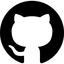
\includegraphics[scale=0.09]{github-icon.png}
          \href{https://github.com/nhejazi}{nhejazi} \\
        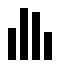
\includegraphics[scale=0.12]{homepage.png}
          \href{https://nimahejazi.org}{nimahejazi.org} \\
        
\includegraphics[scale=0.12]{pdf-icon.png}
        \href{https://bit.ly/2019\_bioc\_modtmle}{bit.ly/2019\_bioc\_modtmle}\\
        Joint work with Alan Hubbard and Mark van der Laan
    \end{minipage}%
    \begin{minipage}{0.35\textwidth}
      \centering
      
\includegraphics[height=0.80in,width=0.80in]{ucberkeleyseal_874_540.eps}
    \end{minipage}
  \end{figure}
}

\date{25 June 2019}

%%%%%%%%%%%%%%%%%%%%%%%%%%%%%%%%%%%%%%%%%%%%%%%%%%%%%%%%%%%%%%%%%%%%%%%%%%%%%%%%

\begin{document}

\begin{frame}[noframenumbering]
  \thispagestyle{empty}
  \titlepage
\end{frame}

%%%%%%%%%%%%%%%%%%%%%%%%%%%%%%%%%%%%%%%%%%%%%%%%%%%%%%%%%%%%%%%%%%%%%%%%%%%%%%%%

\begin{frame}[c,noframenumbering]{Preview}
\thispagestyle{empty}
\begin{center}
\begin{enumerate}
  \itemsep12pt
  \item Model misspecification seriously undermines the utility of many common
    statistical modeling approaches.
  \item Non/semi-parametric theory allows the construction of robust estimators
    that accommodate the use of machine learning.
  \item Moderated variance estimators augment hypothesis testing strategies to
    reduce false positives in small-sample settings.
  \item The moderation approach pioneered by the \texttt{limma} \texttt{R}
    package may easily be extended to non/semi-parametric estimators.
\end{enumerate}
\end{center}

\note{We'll go over this summary again at the end of the talk. Hopefully, it
      will all make more sense then.
}
\end{frame}

%%%%%%%%%%%%%%%%%%%%%%%%%%%%%%%%%%%%%%%%%%%%%%%%%%%%%%%%%%%%%%%%%%%%%%%%%%%%%%%%

\begin{frame}[c]{Data structure and notation}
\begin{center}
\begin{itemize}
  \itemsep12pt
  \item Consider a nonparametric structural equation model (NPSEM) to describe
    observed data $O$ \citep{pearl2000causality}:
    \begin{equation*}\label{npsem}
        W = f_W(U_W); A = f_A(W, U_A); Y = f_Y(A, W, U_Y).
      \end{equation*}
  \item $f_W$, $f_A$, $f_Y$ are flexible but deterministic functions; $U_W$,
    $U_A$, $U_Y$ are exogenous RVs specifying unobserved errors.
  \item Data on a single unit $O = (W, A, Y)$, where $O \sim P_0 \in
    \mathcal{M}$. Observe $O_1, \ldots, O_n$, i.e., $n$ i.i.d.~copies of $O$.
  \item $Y = (Y_b: b = 1, \ldots B)$ is a vector of biomarker outcomes.
\end{itemize}
\end{center}

\note{
}
\end{frame}

%%%%%%%%%%%%%%%%%%%%%%%%%%%%%%%%%%%%%%%%%%%%%%%%%%%%%%%%%%%%%%%%%%%%%%%%%%%%%%%%

\begin{frame}[c]{Interventions and causal inference}
\begin{center}
\begin{itemize}
  \itemsep12pt
  \item NPSEM: time-ordering and counterfactual RV distributions.
  \item \textit{Static intervention} replaces $f_A$ with an assigned value
    $A = a$.
  \item Generates a counterfactual RV $Y(a) = (Y_b^{a}, b: 1, \ldots B)$:
    expression of $B$ biomarkers when $A$ is set to $a$.
  \item Thus, we have potential outcomes $Y_b(1)$ (for $\text{do}(A=1)$) and
    $Y_b(0)$ (for $\text{do}(A=0)$) \citep{rubin2005causal}.
  \item We've now just about defined a canonical causal parameter, the ATE:
    $\psi_b = \E_W[Y_b(1) - Y_b(0)]$ \citep{pearl2000causality}.
\end{itemize}
\end{center}

\note{Statistical parameter may be viewed as a simple adjusted difference in
  means even when identifiability conditions appear unsatisfiable.
}
\end{frame}

%%%%%%%%%%%%%%%%%%%%%%%%%%%%%%%%%%%%%%%%%%%%%%%%%%%%%%%%%%%%%%%%%%%%%%%%%%%%%%%%


\begin{frame}[c]{A familiar workhorse: the linear model}
\begin{center}
\begin{itemize}
  \itemsep12pt
  \item The linear model is \textit{semiparametric} --- linear in parameters!
  \item Flexible: accommodate transformations, interactions, etc.
  \item For each biomarker ($b = 1, \ldots, B$), fit a \textit{working} linear
    model.
  \item Under the working model, the parameter $\beta_b$ captures the ATE,
    allowing construction of estimators and inference.
  \item Test the coefficent of interest using a standard t-test:
    \[ t_{b} = \frac{\hat{\beta}_{b} - \beta_{b, H_0}}{s_b} \]
\end{itemize}
\end{center}

\note{There's nothing particularly wrong with this approach. It's exactly what
      we would come up with after a first-year statistics course. In practice,
      there are many issues: (1) we are forced to specify a functional form, the
      linear model; (2) we end up with unstable variance estimates that sharply
      increase the number of false positives detected, even after multiple
      testing corrections. In practice, the incredible flexibility of the linear
      mode is rarely taken advantage of --- scientific guidance is usually
      lacking to justify the fitting of richer models.
}
\end{frame}

%%%%%%%%%%%%%%%%%%%%%%%%%%%%%%%%%%%%%%%%%%%%%%%%%%%%%%%%%%%%%%%%%%%%%%%%%%%%%%%%

\begin{frame}[c]{Variance moderation robustifies inference}

\begin{center}
\begin{itemize}
  \itemsep12pt
  \item When the sample size is small, $s^2_b$ may be so small that even small
    effects ($\hat{\beta}_{b} - \beta_{b, H_0}$) lead to large $t_{b}$.
  \item This results in false positives. Smyth proposes we get around this by an
    empirical Bayes shrinkage of the $s^2_b$.
  \item Test the coefficent of interest with a \textbf{moderated} t-test:
    \[
      \tilde{t}_{b} = \frac{\hat{\beta}_{b} - \beta_{b, H_0}}{\tilde{s}_b}
      \quad \text{where} \quad
      \tilde{s}^2_b = \frac{s^2_bd_b + s^2_0d_0}{d_b + d_0}
    \]
  \item Eliminates large t-statistics arising merely from very small $s_b$.
\end{itemize}
\end{center}

\note{The substantive contribution here is the use of an empirical Bayes method
      to shrink the standard deviation across all of the biomarkers such that we
      obtain a larger (but accurate) estimate that reduces the number of test
      statistics that are marked as significant by low $s^2_b$ estimates alone.

      Note that this is \textbf{not} the exact formulation of the moderated
      t-statistic as given by Smyth (his derivation assumes a hierarchical
      model; see original paper if interested). This formulation does a good
      enough job to help us see the bigger picture.
}
\end{frame}

%%%%%%%%%%%%%%%%%%%%%%%%%%%%%%%%%%%%%%%%%%%%%%%%%%%%%%%%%%%%%%%%%%%%%%%%%%%%%%%%

\begin{frame}[c]{Variable importance measures as target parameters}

\begin{center}
\begin{itemize}
  \itemsep12pt
  \item If the working model is incorrect, $\beta_b$ does not correspond to the
    ATE --- thus leading to biased results.
  \item The statistical functional identifying the ATE may be used as a variable
    importance measure (VIM):
    \[ \Psi_b(P_0) = \mathbb{E}_{W,0}[\mathbb{E}_0[Y_b \mid A = 1, W] -
      \mathbb{E}_0[Y_b \mid A = 0, W]] \]
  \item One-step and targeted minimum loss estimation build efficient, doubly
    robust estimators $\Psi_b(P_n^{\star})$ of $\Psi_b(P_0)$.
\end{itemize}
\end{center}

\note{By allowing scientific questions to inform the parameters that we choose
      to estimate, we can do a better job of actually answering the questions of
      interest to our collaborators. Further, we abandon the need to specify the
      functional relationship between our outcome and covariates; moreover, we
      can now make use of advances in machine learning.
}
\end{frame}

%%%%%%%%%%%%%%%%%%%%%%%%%%%%%%%%%%%%%%%%%%%%%%%%%%%%%%%%%%%%%%%%%%%%%%%%%%%%%%%%

\begin{frame}[c]{Robust and locally efficient estimation}

\begin{center}
\begin{itemize}
  \itemsep12pt
  \item Asymptotic linearity:
    \[ \Psi_b(P_n^{\star}) - \Psi_b(P_0) = \frac{1}{n} \sum_{i = 1}^{n}
      D_b(O_i) + o_P\left(\frac{1}{\sqrt{n}}\right) \]
  \item The influence function $D_b$ for the ATE takes the form
    \begin{align*}
      D_b (O_i) =& \left[\frac{2A_i - 1}{g_0(A_i \mid W_i)} \right] (Y_{b, i} -
      Q_{0,b}(A_i, W_i))\\ &+ Q_{0,b}(1, W_i) - Q_{0,b}(0, W_i) - \Psi_b,
    \end{align*}
    where $g_0(A \mid W) = \mathbb{P}_0(A = 1 \mid W)$ is the treatment
    mechanism and $Q_{0,b}(A,W) = \mathbb{E}_0[Y_b \mid A, W]$ is the outcome
    model.
\end{itemize}
\end{center}

\note{Natural use of machine learning methods for the estimation of both $Q_0$
      and $g_0$. Focuses effort to achieve minimal bias and asymptotic
      semiparametric efficiency bound for the variance, but still get inference
      (with some assumptions).
}
\end{frame}

%%%%%%%%%%%%%%%%%%%%%%%%%%%%%%%%%%%%%%%%%%%%%%%%%%%%%%%%%%%%%%%%%%%%%%%%%%%%%%%%

\begin{frame}[c]{Robust and locally efficient estimation}

\begin{center}
\begin{itemize}
  \itemsep12pt
  \item wrt the data $O = (W,A,Y)$, $D_b(O)$ admits an orthogonal decomposition
    --- i.e.,$D_b(O) = D_b^Y(O) + D_b^A(O) + D_b^W(O)$.
  \item Under randomization, $D_b^A(O) = 0$ and need not be estimated, though
    estimation improves overall efficiency \citep{tsiatis2007semiparametric}.
  \item No need to specify functional forms or assume we know the model
    underlying the true data-generating distribution $P_0$.
  \item Machine learning to estimate nuisance functions $g_0(A \mid W)$ and
    $Q_{0,b}(A,W)$, e.g., via stacked regression or cross-validation selectors
    \citep{breiman1996stacked, vdl2007super}.
\end{itemize}
\end{center}

\note{Natural use of machine learning methods for the estimation of both $Q_0$
      and $g_0$. Focuses effort to achieve minimal bias and asymptotic
      semiparametric efficiency bound for the variance, but still get inference
      (with some assumptions).
}
\end{frame}

%%%%%%%%%%%%%%%%%%%%%%%%%%%%%%%%%%%%%%%%%%%%%%%%%%%%%%%%%%%%%%%%%%%%%%%%%%%%%%%%

\begin{frame}[c]{Robust inference via the influence function}

\begin{center}
\begin{itemize}
  \itemsep12pt
  \item Suppose we have estimated $g_0(A \mid W)$ and $Q_{0,b}(A,W)$ via ML,
    yielding an estimate $D_{n,b}(O)$ of $D_b(O)$, for $b = 1, \ldots, B$.
  \item Conservative variance estimator for $\Psi_b(P_n^{\star})$ based on
    $D_{n,b}(O)$:
    \begin{equation*}
      se_b = \sqrt{\frac{s^2(D_{n,b})}{n}} \quad \text{where} \quad
      s^2(D_{n,b}) = \frac{1}{n}\sum_{i=1}^n\left(D_{n,b}(O_i) \right)^2
    \end{equation*}
  \item Under $H_0: \Psi_b(P_0) = 0$ (no treatment effect), test statistic:
    \begin{equation*}
      t_b = \frac{\Psi_b(P_n^{\star})}{se_b}
    \end{equation*}
\end{itemize}
\end{center}

\note{Using the influence curve representation, we can obtain all of the
  standard objects of statistical interest, but for more interesting parameters.
}
\end{frame}

%%%%%%%%%%%%%%%%%%%%%%%%%%%%%%%%%%%%%%%%%%%%%%%%%%%%%%%%%%%%%%%%%%%%%%%%%%%%%%%%

\begin{frame}[c]{Moderated statistics based on influence functions}

\begin{center}
\begin{itemize}
  \itemsep12pt
  \item Moderated t-statistic of~\cite{smyth2004linear} naturally extends to
    locally efficient estimators:
    \begin{equation*}
      \tilde{t}_b = \frac{\Psi_b(P_n^{\star})}{\widetilde{se}_b}
    \end{equation*}
    where the posterior estimate of influence function variance is
    \begin{equation*}
      \tilde{s}^2_b = \frac{s^2_b(D_{n,b}) d_b + s^2_0 d_0}{d_b + d_0}
    \end{equation*}
  \item Preserves robust variance estimator but adds stability that smoothens
    its small-sample behavior.
\end{itemize}
\end{center}

\note{
  \begin{itemize}
    \item Consider this is repeated for $b = 1, \ldots, B$  different
      biomarkers, so that one has, for each $b$:
      $$\Psi_b(Q_{b,n}^{*}), S_b^2(IC_{b,n}),$$
      estimate of variable importance and standard error for all $B$.
    \item Propose an existing joint-inferential procedure that can add some
      finite-sample robustness to an estimator that can be highly variable.
   \end{itemize}
}
\end{frame}

%%%%%%%%%%%%%%%%%%%%%%%%%%%%%%%%%%%%%%%%%%%%%%%%%%%%%%%%%%%%%%%%%%%%%%%%%%%%%%%%

\begin{frame}[c]{That's nice and all but where's the proof?}

\begin{center}
\begin{itemize}
  \item Simulation study under two settings: (1) global null and (2) when half
    of probes respond to treatment.
    \begin{align*}
      W_1 &\sim \text{Unif}(0, 1);
      W_2 \sim \text{Unif}(0, 1)\\
      A &\sim \text{Bern}\left(\text{expit}(-1.2 - 2.5 \cdot W_1 + 3.5 \cdot
        W_2)\right) \\
      Y_{\text{null}} &= 2 + 5 \cdot W_1 + 0.5 \cdot W_2 + W_1 \cdot W_2 +
        \epsilon\\
      Y_{\text{non-null}} &= 2 + 5 \cdot W_1 + 0.5 \cdot W_2 + W_1 \cdot W_2 +
        5 \cdot A + \epsilon,
    \end{align*}
  \item Data-adaptive estimation of relevant nuisance quantities.
  \item Compares TML estimator of ATE to working linear model, under moderated
    and standard variance estimates.
\end{itemize}
\end{center}

\note{Essentially, we have the same concerns about using variable importance
  measures that we did about using the standard t-test --- that is, non-robut
  estimates of the standard error of the estimator of the target parameter can
  cause erroneous identification of biomarkers (false positives). To reduce
  this, we can apply the same machinery that we did in the case of the standard
  t-test for our naive linear modeling approach.
}
\end{frame}

%%%%%%%%%%%%%%%%%%%%%%%%%%%%%%%%%%%%%%%%%%%%%%%%%%%%%%%%%%%%%%%%%%%%%%%%%%%%%%%%

\begin{frame}[c]{That's nice and all but where's the proof? Global null.}

\centering
\includegraphics[origin=c,scale=0.25]{vis_fdr_sl_null_logistic}

\note{
  \begin{itemize}
    \item Control of the FDR using the Benjamini-Hochberg
      correction applied to the results of hypothesis tests based on
      \texttt{limma}, standard TML estimator without variance moderation, and
      TML estimator with variance moderation.
  \item TML estimators converges to the correct FDR asymptotically and achieves
    the nominal rate by $n = 250$ while the moderated linear model does not
    exhibit correct control of the FDR.
  \end{itemize}
}
\end{frame}

%%%%%%%%%%%%%%%%%%%%%%%%%%%%%%%%%%%%%%%%%%%%%%%%%%%%%%%%%%%%%%%%%%%%%%%%%%%%%%%%

\begin{frame}[c]{That's nice and all but where's the proof? Treatment effect.}

\centering
\includegraphics[origin=c,scale=0.25]{vis_fdr_sl_findings_logistic}

\note{
  \begin{itemize}
    \item Control of the FDR using the Benjamini-Hochberg correction applied to
      the results of hypothesis tests based on the moderated linear modeling
      approach of \texttt{limma}, the standard TML estimator without any
      variance moderation, and the TML estimator with variance moderation.
      Application of TML estimators converges to the correct FDR asymptotically
      and achieves the nominal rate by $n = 250$ while the moderated linear
      model does not exhibit correct control of the FDR.
  \end{itemize}
}
\end{frame}

%%%%%%%%%%%%%%%%%%%%%%%%%%%%%%%%%%%%%%%%%%%%%%%%%%%%%%%%%%%%%%%%%%%%%%%%%%%%%%%%

\begin{frame}[c]{Software implementation: \texttt{R/biotmle}}

\begin{center}
\begin{itemize}
  \itemsep12pt
  \item \texttt{R} package for DE analysis based on TML estimators of the ATE
    that use machine learning for $g_0(A \mid W)$ and $Q_{0,b}(A,W)$.
  \item Statistical inference based on \textit{moderated} variance estimator.
  \item Check out the package:
    \begin{itemize}
      \itemsep8pt
      \item \url{https://github.com/nhejazi/biotmle}
      \item \url{https://bioconductor.org/packages/biotmle}
    \end{itemize}
\end{itemize}
\end{center}

\note{Use it. File an issue. Help make it better!
}
\end{frame}

%%%%%%%%%%%%%%%%%%%%%%%%%%%%%%%%%%%%%%%%%%%%%%%%%%%%%%%%%%%%%%%%%%%%%%%%%%%%%%%%

\begin{frame}[c]{The \texttt{tlverse} for Targeted Learning}

\begin{figure}[H]
  \centering
  
\includegraphics[width=\textwidth]{tlverse}
  \caption{
    \url{https://github.com/tlverse}
  }
\end{figure}
\begin{itemize}
  \itemsep12pt
  \item An ecosystem of \texttt{R} packages for Targeted Learning, all sharing a
    core set of design principles centered on extensibility.
  \item \textit{Draft phase} Targeted Learning handbook:
    \url{https://tlverse.org/tlverse-handbook}
\end{itemize}

\note{Use it. File issues. Help make it better!
}
\end{frame}


%%%%%%%%%%%%%%%%%%%%%%%%%%%%%%%%%%%%%%%%%%%%%%%%%%%%%%%%%%%%%%%%%%%%%%%%%%%%%%%%

\begin{frame}[c]{Review}
\begin{center}
\begin{enumerate}
  \itemsep12pt
  \item Model misspecification seriously undermines the utility of many common
    statistical modeling approaches.
  \item Non/semi-parametric theory allows the construction of robust estimators
    that accommodate the use of machine learning.
  \item Moderated variance estimators augment hypothesis testing strategies to
    reduce false positives in small-sample settings.
  \item The moderation approach pioneered by the \texttt{limma} \texttt{R}
    package may easily be extended to non/semi-parametric estimators.
\end{enumerate}
\end{center}


\note{It's always good to include a summary.}
\end{frame}

%%%%%%%%%%%%%%%%%%%%%%%%%%%%%%%%%%%%%%%%%%%%%%%%%%%%%%%%%%%%%%%%%%%%%%%%%%%%%%%%

\begin{frame}[c,allowframebreaks]{}

\small
\bibliographystyle{apalike}
%\nocite{*}
\bibliography{references}

\end{frame}

%%%%%%%%%%%%%%%%%%%%%%%%%%%%%%%%%%%%%%%%%%%%%%%%%%%%%%%%%%%%%%%%%%%%%%%%%%%%%%%%

\begin{frame}[c]{Thank you, Bioconductor.}

\large
Slides: \href{https://bit.ly/2019\_bioc\_modtmle}{bit.ly/2019\_bioc\_modtmle}
  \quad

\includegraphics[height=4mm]{Figs/cc-zero.png}

\vspace{2mm}
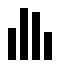
\includegraphics[scale=0.14]{homepage.png} \url{https://nimahejazi.org}

\vspace{2mm}
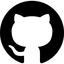
\includegraphics[scale=0.11]{github-icon.png}
  \url{https://github.com/nhejazi}

\vspace{2mm}

\includegraphics[scale=0.14]{twitter-icon.png}
  \url{https://twitter.com/nshejazi}

\note{Here's where you can find me, as well as the slides for this talk.}

\end{frame}

\end{document}
